\documentclass{article}

% if you need to pass options to natbib, use, e.g.:
%     \PassOptionsToPackage{numbers, compress}{natbib}
% before loading neurips_2021

% ready for submission
\usepackage[preprint]{neurips_2023}

% to compile a preprint version, e.g., for submission to arXiv, add add the
% [preprint] option:
%     \usepackage[preprint]{neurips_2021}

% to compile a camera-ready version, add the [final] option, e.g.:
%     \usepackage[final]{neurips_2021}

% to avoid loading the natbib package, add option nonatbib:
%    \usepackage[nonatbib]{neurips_2021}

\usepackage[utf8]{inputenc} % allow utf-8 input
\usepackage{bm}

\usepackage[T1]{fontenc}    % use 8-bit T1 fonts
\usepackage[colorlinks=true]{hyperref}       % hyperlinks
\usepackage{url}            % simple URL typesetting
\usepackage{booktabs}       % professional-quality tables
\usepackage{amsfonts}       % blackboard math symbols
\usepackage{nicefrac}       % compact symbols for 1/2, etc.
\usepackage{microtype}      % microtypography
\usepackage{xcolor}         % colors
\usepackage{graphicx}
\usepackage{cleveref}
\usepackage{wrapfig}
\usepackage{mwe}
\usepackage{caption}

\title{Corporate vs. Academia: Who Dominates Computer Vision Conferences?}

% The \author macro works with any number of authors. There are two commands
% used to separate the names and addresses of multiple authors: \And and \AND.
%
% Using \And between authors leaves it to LaTeX to determine where to break the
% lines. Using \AND forces a line break at that point. So, if LaTeX puts 3 of 4
% authors names on the first line, and the last on the second line, try using
% \AND instead of \And before the third author name.

\author{
  \small Irem Karaca\thanks{Matrikelnummer 6939373, \texttt{irem.karaca@student.uni-tuebingen.de}}\\
  % \small Matrikelnummer 6939373\\
  % \small \texttt{@student.uni-tuebingen.de} \\
  \And
  \small Merve Kocabas\thanks{Matrikelnummer 7040890, \texttt{merve.kocabas@student.uni-tuebingen.de}}\\
  % \small Matrikelnummer 7040890\\
  % \small \texttt{merve.kocabas@student.uni-tuebingen.de} \\
  \And
  \small Hari Joshithaa Aghilah Senthilprathiban\thanks{Matrikelnummer 6943473, \texttt{hari-joshitha.aghilah-senthilprathiban@student.uni-tuebingen.de}}\\
  % \small Matrikelnummer 6943473\\
  % \small \texttt{hari-joshitha.aghilah-senthilprathiban@student.uni-tuebingen.de} \\
  \And
  \small Shubham S. Raheja\thanks{Matrikelnummer 7001572, \texttt{shubham.raheja@student.uni-tuebingen.de}}\\
  % \small Matrikelnummer 7001572\\
  % \small \texttt{shubham.raheja@student.uni-tuebingen.de} \\  
}

\begin{document}

\maketitle
\vspace{-10pt}
\begin{abstract}
  % \emph{[Use this abstract to briefly explain what you are planning to do. Here is an example:]} We are planning to use the collection of \href{https://openreview-py.readthedocs.io/en/latest/getting_data.html}{all papers ever \emph{submitted} to the ICLR conference} to see how well paper acceptance can be predicted from trivial features, such as the paper's overall length, number of words or number of figures. We are planning to use logistic regression for this purpose.

Corporate involvement in computer vision research has grown significantly, raising questions about its influence on the field. This study analyzes corporate-affiliated papers in top-tier conferences (CVPR, ICCV, WACV) to assess publication trends, impact, and research focus. While academia still dominates in volume, corporate contributions have steadily increased, reaching record levels. Industry papers receive higher citations on average and are concentrated among a few large tech firms. Corporate research leans toward high-impact and applied areas while academia emphasizes theoretical foundations. These trends highlight the need for stronger academic-industry collaboration and open research initiatives to maintain a balanced research landscape.

\end{abstract}
\vspace{-10pt}
% You can find a detailed example and instructions on how to use this style file in the attached \texttt{neurips\_2023.tex} file. This includes instructions for how to lay out citations.

\section{Introduction}
\vspace{-7pt}
Computer vision is a rapidly growing field that plays a crucial role in advancing AI. Leading conferences such as CVPR, ICCV, and WACV serve as key venues for presenting cutting-edge research. The increasing participation of corporate entities in these conferences raises important questions about their influence on the field’s development and direction.

Research indicates that corporate involvement in AI publications, particularly in computer vision, is substantial. Färber et al. identify computer vision as the AI domain with the highest corporate engagement[1], while Ye finds that dual-affiliated AI researchers tend to receive higher citations[2]. Building on these insights, this study examines the extent of corporate participation in major computer vision conferences and its broader impact.

We first analyze trends in corporate-affiliated publications to assess industry involvement over time. Next, we explore citation metrics to compare the influence of corporate and academic papers. We then categorize corporate contributions by company size, considering how large technology firms may shape research priorities. Finally, we examine keyword trends to identify differences in research focus between industry and academia. These analyses provide a comprehensive understanding of corporate influence on computer vision research and its implications for the field’s trajectory.
\vspace{-7pt}
\section{Data and Methods}
\vspace{-7pt}
This study focuses on the most influential computer vision conferences that attract high-quality submissions from academia and industry. CVPR (held annually) and ICCV (biennial), ranked \#1 and \#2 on Google Scholar Best Computer Science Conferences in Computer Vision list [3], are ideal venues for analyzing corporate and academic contributions. WACV (\#9) is included for its emphasis on applied research, contrasting with the more theoretical nature of CVPR and ICCV.

We construct our dataset by extracting paper titles, authors, and affiliations using Paper Copilot GitHub [4]. Since CVPR, ICCV, and WACV proceedings are published on IEEE Xplore, we use paper titles to scrape their respective IEEE Xplore pages, collecting 
% \begin{figure}
%     \noindent
%     \hspace{-2mm}
%     \begin{minipage}{0.5\textwidth} 
%         \centering
%         \vspace{-30pt}
%         \setlength{\tabcolsep}{3pt} % Reduce column spacing
%         \begin{tabular}{|c|c|c|c|}
%         \hline
%         \textbf{Category} & \textbf{Turnover}  & \textbf{Employee count} & \textbf{Growth rate} \\ \hline
%         \textbf{Big}      & \textgreater{}\$1B & \textgreater{}5,000     & \textless{}10\%      \\ \hline
%         \textbf{Mid-size} & \$100M–\$1B          & 500–5,000               & 10–20\%              \\ \hline
%         \textbf{Scaleup}  & \$10M–\$100M         & 50–500                  & \textgreater{}20\%   \\ \hline
%         \textbf{Startup}  & \textless{}\$10M   & \textless{}50           & \textgreater{}50\%   \\ \hline
%         \end{tabular}
%         \begin{minipage}{1.2\textwidth}
%             \centering
%         \caption{\hspace{1mm}Corporate size categorization cutoff values for}
%             \vspace{-7pt}
%             \caption*{turnover, employee count, and growth rate.}
%             \label{fig:corporate_size}
%         \end{minipage}
%     \end{minipage}
%     \vspace{-24pt}
% \end{figure}

\begin{wraptable}{r}{0.5\textwidth} % Right-aligned, 50% text width
    \vspace{-20pt} % Adjust vertical spacing to fit well
    \setlength{\tabcolsep}{3pt} % Reduce column spacing
    \centering
    \begin{tabular}{|c|c|c|c|}
        \hline
        \textbf{Category} & \textbf{Turnover}  & \textbf{Employee count} & \textbf{Growth rate} \\ \hline
        \textbf{Big}      & \textgreater{}\$1B & \textgreater{}5,000     & \textless{}10\%      \\ \hline
        \textbf{Mid-size} & \$100M–\$1B        & 500–5,000               & 10–20\%              \\ \hline
        \textbf{Scaleup}  & \$10M–\$100M       & 50–500                  & \textgreater{}20\%   \\ \hline
        \textbf{Startup}  & \textless{}\$10M   & \textless{}50           & \textgreater{}50\%   \\ \hline
    \end{tabular}
    
    \captionsetup{skip=2pt} % Reduce vertical space between caption lines
    \caption{\hspace{1mm}Corporate size categorization cutoff values for turnover, employee count, and growth rate.}
    \vspace{-7pt} % Reduce space before next caption line
    \caption*{} % Non-numbered caption
    \label{tab:corporate_size}
    \vspace{-10pt} % Adjust space below the table
\end{wraptable}


\begin{wrapfigure}{r}{0.38\textwidth}
\vspace{-100pt}
\centering
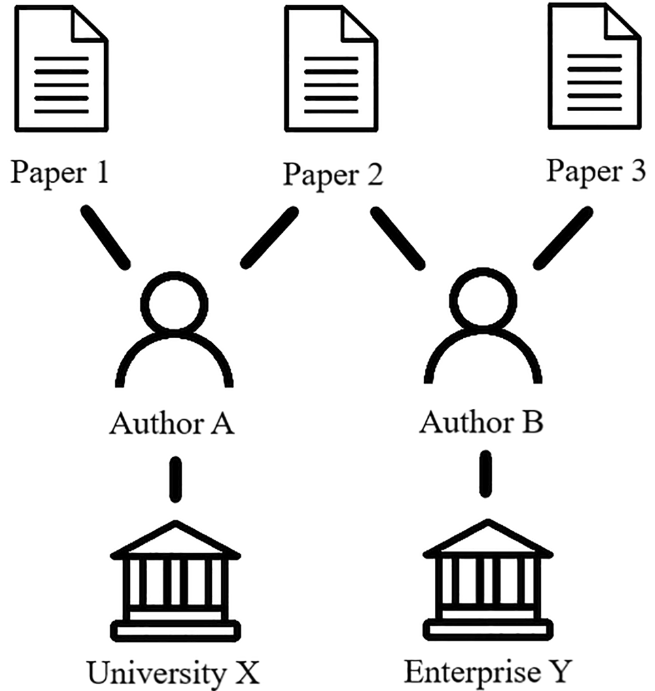
\includegraphics[width=.95\linewidth]{report/images/affiliation-combination.png}
\caption{Illustration of different paper-author-affiliation relationships[1]. Authors with both corporate and academic affiliations have their contributions split proportionally. Papers with any corporate-affiliated authors are classified as corporate-affiliated, while those with $\geq$ 50\% corporate contributions are considered corporate-led.}
\vspace{-10pt}
% Authors with both corporate and academic affiliations have their contributions split proportionally. Papers with any corporate-affiliated authors are classified as corporate-affiliated, while those with $\geq$ 50\% corporate contributions are considered corporate-led.
\label{fig:affiliation-combination}
\vspace{-20pt}
\end{wrapfigure}
citation counts (IEEE  and other publishers) and IEEE keywords. Our dataset, spanning 2019 to 2024, includes 18,925 papers, with 45\% from CVPR, 35\% from ICCV, and 20\% from WACV. This period allows us to analyze citation trends, acknowledging that older papers (e.g., from 2019) tend to have higher citation counts due to accumulation over time.

Each paper is categorized based on author affiliations, as shown in Figure \ref{fig:affiliation-combination}. Corporates are categorized utilizing Table \ref{tab:corporate_size} and Dun \& Bradstreet Business Directory [5]. Papers are further classified into 17 research categories using arXiv taxonomy [6] and ChatGPT. The dataset and additional resources are available at: \url{https://github.com/mervekocabas/Data_Literacy}.


% \subsection{Spearman's Rank Correlation Coefficient}
% To analyze the temporal trend in the proportion of corporate-affiliated papers presented at conferences, we employed Spearman's Rank Correlation Coefficient ($\rho_s$), a non-parametric statistical method suitable for detecting monotonic relationships in time series data [7]. This method is effective for small datasets and does not require the assumption of normally distributed variables [8]. Spearman's $\rho_s$ is calculated using the following equation:
% \begin{equation}
% \rho_s = 1 - \frac{6 \sum d_i^2}{n(n^2 - 1)}
% \end{equation}
% where $d_i$ is the difference between the ranks of corresponding values in the two variables, and $n$ is the number of observations. The coefficient ranges from $-1$ to $1$, where closer to $1$ indicate a strong positive monotonic relationship, values closer to $-1$ indicate a strong negative monotonic relationship, and values near $0$ indicate no monotonic relationship. To assess the statistical significance of the observed correlation, a significance test by computing the p-value is conducted. A p-value less than a predetermined significance level (0.05) indicates that the observed correlation is statistically significant, implying that the relationship between the variables is unlikely to have occurred by chance.

% \subsection{Mann-Whitney U test}
% To analyze the IEEE citations in corporate co-authored papers and academia papers which do not have a normal distribution, one sided Mann-Whitney U test is used. The Mann-Whitney U test compares two independent samples by ranking all observations together and summing the ranks for each group [9]. The U statistic measures how often a value in one group is greater than a value in the other is calculated as follows,
% \begin{equation}
% U_x = n_xn_y\frac{n_x(n_x+1)}{2}-R_1
% \end{equation}
% \begin{equation}
%     U_y = n_xn_y\frac{n_y(n_y+1)}{2}-R_2
% \end{equation}
% where $n_x$ and $n_y$ are the sample sizes for both the groups and $R_1$ and $R_2$ are the rank sums for both the groups respectively. Under the null hypothesis, the distribution of \( U \) is approximately normal with mean $\mu_U$ and standard deviation $\sigma_U$ as follows,
% \begin{equation}
%     \mu_U = \frac{n_x n_y}{2}
% \end{equation}
% \begin{equation}
%     \sigma_U = \sqrt{\frac{n_x n_y (n_x + n_y + 1)}{12}}
% \end{equation}
% \begin{equation}
%     Z = \frac{U - \mu_U}{\sigma_U} = \frac{U - \frac{n_x n_y}{2}}{\sqrt{\frac{n_x n_y (n_x + n_y + 1)}{12}}}
% \end{equation}
% where $U$ is either $U_x$ or $U_y$. The z-score $Z$ is compared to a critical value $\alpha$ to determine statistical significance, leading to either acceptance or rejection of the null hypothesis [9].


% \clearpage
\vspace{-7pt}
\section{Results}
\vspace{-7pt}
\subsection{Growth of Corporate-Affiliated Research}
\vspace{-7pt}
To investigate whether corporate-affiliated research has gained influence at top-tier computer vision conferences, we begin by analyzing the trend in corporate-affiliated paper contributions over time. As shown in Figure \ref{fig:corporate_ratio_graph}, the proportion of corporate-affiliated papers has steadily increased across major computer vision conferences (CVPR, ICCV, and WACV). This trend suggests that corporate involvement in these venues has expanded significantly in recent years. Despite this rise, academia remains the dominant contributor. Even at its highest level, corporate affiliation does not exceed 47\% of total papers. Notably, ICCV and CVPR exhibit higher levels of corporate participation compared to WACV, which consistently lags in corporate representation. To quantify this trend, we applied Spearman rank correlation analysis (Figure  \ref{fig:corporate_ratio_graph}). We opted for Spearman correlation because our dataset contains a limited and small number of time points[7] with 6 years, and we are analyzing a temporal trend where a monotonic relationship is expected rather than a strictly linear one[8]. The results reveal that there exits a significant monotonic increasing relationship. These findings reinforce the conclusion that corporate presence in computer vision research is experiencing sustained growth within top-tier academic venues.
\vspace{-2pt}
% \begin{figure}[ht]
%   \centering
%   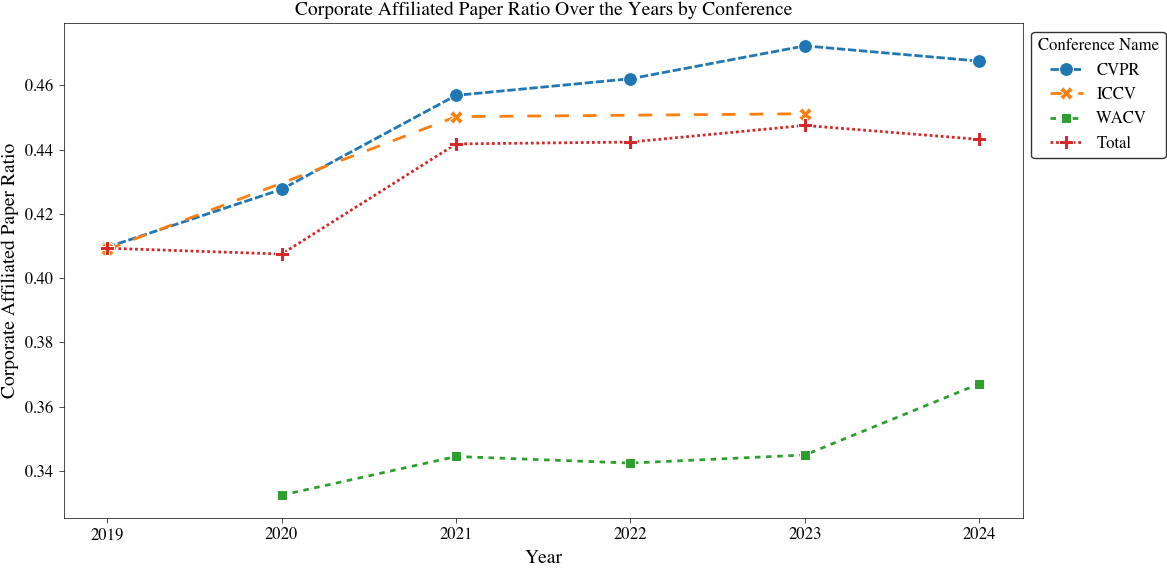
\includegraphics[width=0.6\textwidth]{report/images/corporate_ratio_graph_final.png}  
%   \caption{Corporate affiliated paper ratio over the years for each conference and total dataset.}
%   \label{fig:corporate_ratio_graph}
% \end{figure}

% \begin{table}[ht]
% \centering
% \begin{tabular}{|l|c|c|c|}
% \hline
% \textbf{} & \( \bm{\rho}_\bm{s} \) & \textbf{p-} & {\textbf{Significant}\\ \textbf{}&\textbf{}&\textbf{value}&\textbf{Relationship?}} \\ \hline
% CVPR & 0.94 & 0.01 & Yes \\ \hline
% ICCV & 1.00 & 0.00 & Yes \\ \hline
% WACV & 0.90 & 0.04 & Yes \\ \hline
% Total & 0.88 & 0.02 & Yes \\ \hline
% \end{tabular}
% \caption{Spearman rank correlation results for each conference and total dataset.}
% \label{tab:spearman_results}
% \end{table}

% \begin{figure}[ht]
%   \centering
%   \begin{minipage}{0.5\textwidth}
%     \centering
%     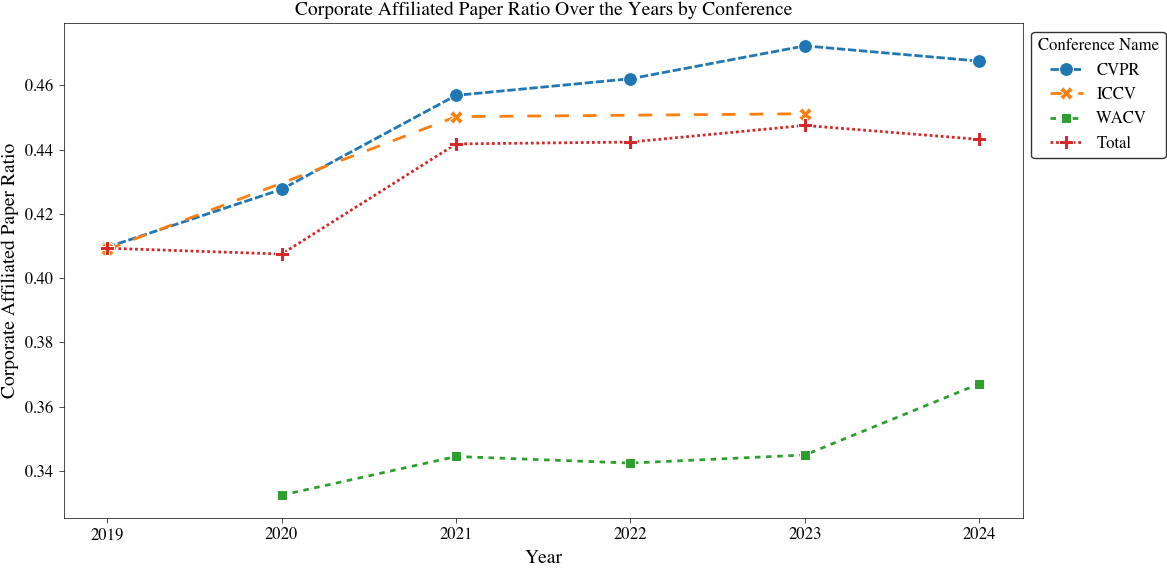
\includegraphics[width=\textwidth]{report/images/corporate_ratio_graph_final.png}
%     \label{fig:corporate_ratio_graph}
%     \vfill  % Fill the vertical space
%   \end{minipage}%
%   \hfill
%   \begin{minipage}{0.3\textwidth}
%     \centering
%     \begin{tabular}{|l|c|c|}
%     \hline
%     \multicolumn{1}{|c|}{} & \textbf{\begin{tabular}[c]{@{}c@{}}Spearman’s Rank \\ Correlation Coefficient\end{tabular}} & \textbf{p-value} \\ \hline
%     CVPR                   & 0.94                                                                                        & 0.01*            \\ \hline
%     ICCV                   & 1.00                                                                                        & 0.00*            \\ \hline
%     WAVCV                  & 0.90                                                                                        & 0.04*            \\ \hline
%     Total                  & 0.88                                                                                        & 0.02*            \\ \hline
%     \end{tabular}
%     \label{tab:spearman_results}
%     \vfill  % Fill the vertical space
%   \end{minipage}

%   % Add a new minipage for captions
%   \vspace{-10pt} % Add some vertical space between the figure and captions
%   \begin{minipage}{0.5\textwidth}
%     \caption{Corporate affiliated paper ratio over the years for each conference and total dataset.}
%     \label{fig:corporate_ratio_graph}
%   \end{minipage}%
%   \hfill

% \end{figure}
\begin{figure}[ht]
    \centering
    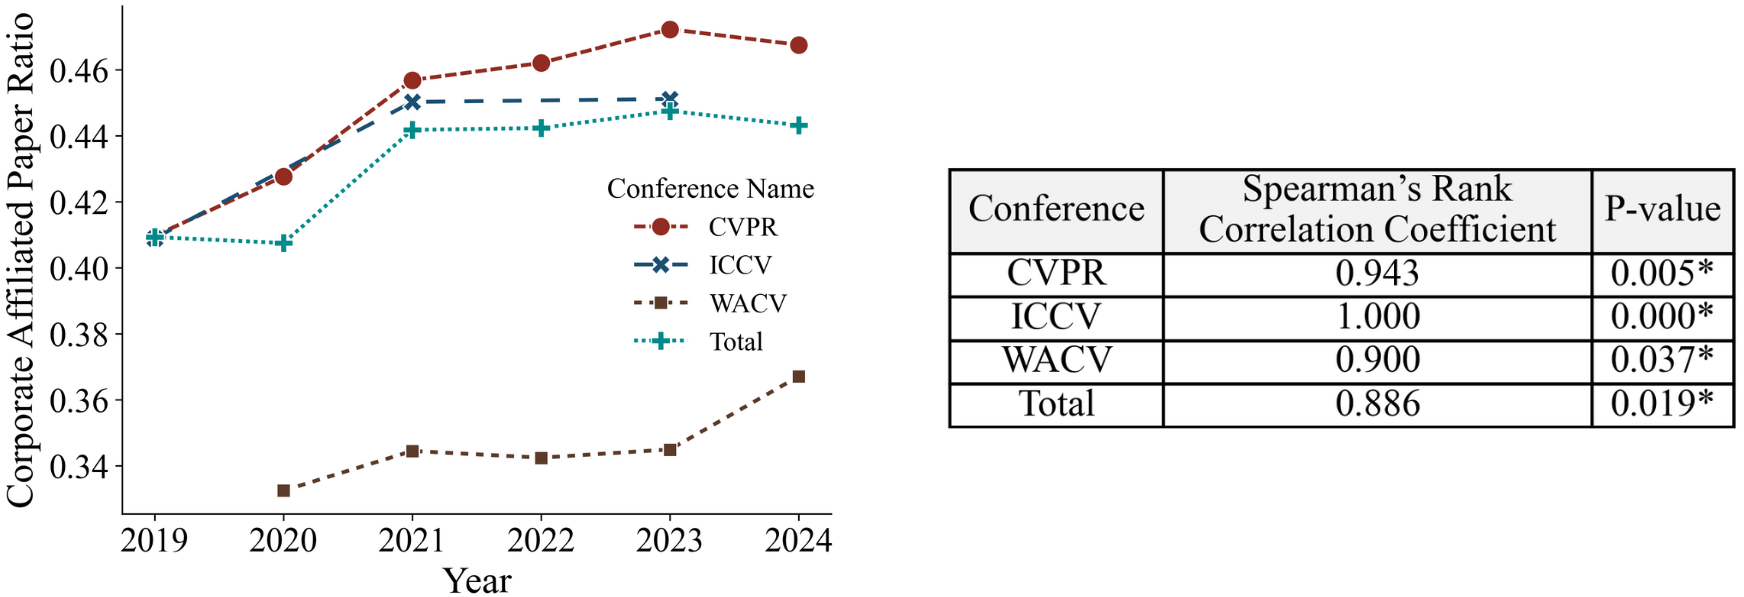
\includegraphics[width=0.9\linewidth]{report/images/corporate_ratio_table.png}
    \caption{The plot on the left shows an increasing trend in corporate contributions, with CVPR and ICCV maintaining higher ratios compared to WACV and reaching record levels in corporate affiliation at last years. The accompanying table on right presents Spearman’s rank correlation coefficients, all of which indicate strong positive correlations (coefficients exceeding 0.88) . Statistically significant values (p < 0.05) are marked with an asterisk (*).}
    \label{fig:corporate_ratio_graph}
    % \vspace{-5pt}
\end{figure}
\vspace{-18pt}
\subsection{Citation Impact of Corporate-Affiliated Research}
\vspace{-7pt}
Beyond their increasing presence, corporate-affiliated papers must also be evaluated in terms of their impact. One widely accepted measure of research influence is citation count, which reflects the extent to which a paper shapes subsequent research. As illustrated in Figure \ref{fig:ieee_citations}, corporate-affiliated papers 
\begin{figure}[ht]
    \centering
    % \vspace{-10pt}
    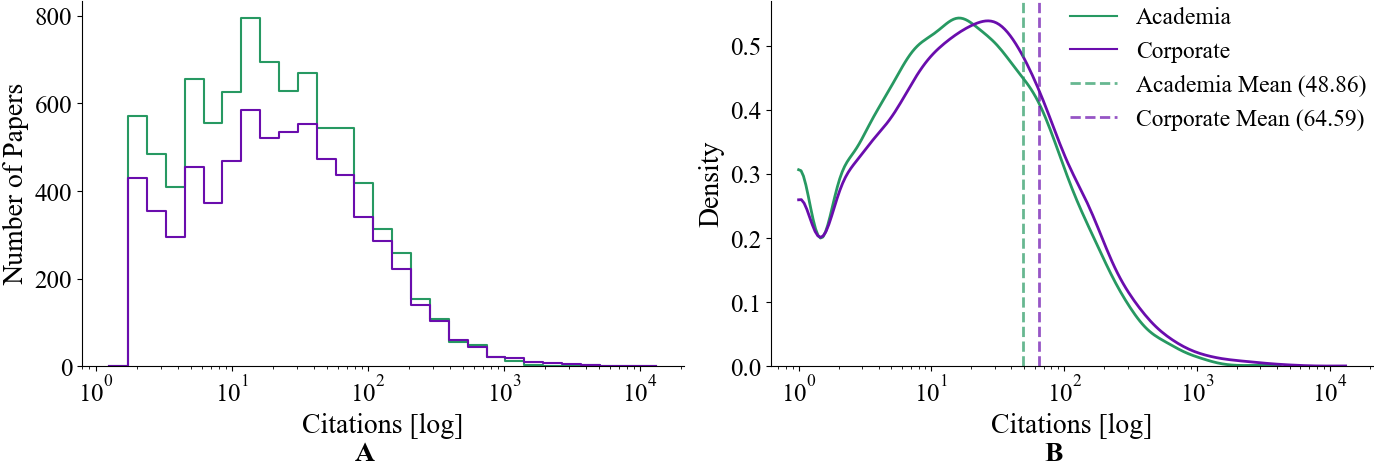
\includegraphics[width=0.9\linewidth]{report/images/ieee_citations.png}
    \caption{Citation distributions of academic and corporate papers show that corporate papers tend to have a higher average number of citations and a wider spread in their citation counts. In contrast, academic papers are more numerous but are generally concentrated in lower citation ranges.}
    \label{fig:ieee_citations}
    \vspace{-10pt}
\end{figure}

exhibit higher average citation counts than academic papers, despite constituting a smaller proportion of total publications. While academic papers are more numerous, their citation distribution is concentrated in the lower ranges, indicating that many receive moderate attention. In contrast, corporate-affiliated papers have a broader citation distribution, suggesting that they are more likely to receive high citation counts. To formally test whether corporate papers have a significantly higher mean citation count ($\mu_2$) than academic papers ($\mu_1$), since the data is not normally distributed we conduct a Mann–Whitney U test[9] with a significance threshold of $\alpha = 0.05$. The null ($H_0$) and alternative ($H_\alpha$) hypotheses are as follows:
\[
H_0 = \mu_2 \leq \mu_1 (\mathrm{Corporate \ papers\ have \ a \ smaller \ or \ equal \ mean \ than \ academia \ papers})
\]
\[
H_\alpha = \mu_2 > \mu_1 (\mathrm{Corporate \ papers\ have \ a \ larger \ mean\ than \ academia \ papers)}
\]
The test results indicate that p-value $\ll 0.05$, allowing us to reject $H_0$. This confirms a statistically significant difference, supporting the conclusion that corporate-affiliated papers tend to achieve higher citation impact compared to their academic counterparts.   
\vspace{-10pt}
\subsection{Influence of Large Corporations}
\vspace{-7pt}
Given the growth and impact of corporate-affiliated research, it is essential to examine the role of large technology companies in driving this trend. As shown in Figure \ref{fig:corporate_size_graph}, large corporations contribute over 60\% of corporate-affiliated papers and nearly 80\% of total corporate research output. This dominance is unsurprising, as cutting-edge computer vision research requires substantial computational resources, proprietary datasets, and advanced machine learning infrastructure—elements that favor well-funded industry research labs. The top 10 most prolific corporations—Google, Facebook, Microsoft, Huawei, Adobe, Tencent, Alibaba, Amazon, Nvidia, and Apple—reinforce this pattern, as all are classified as large-scale tech firms. These findings raise critical questions regarding the degree to which corporate interests shape the overall research agenda in computer vision.

\begin{figure}[ht]
  \centering
  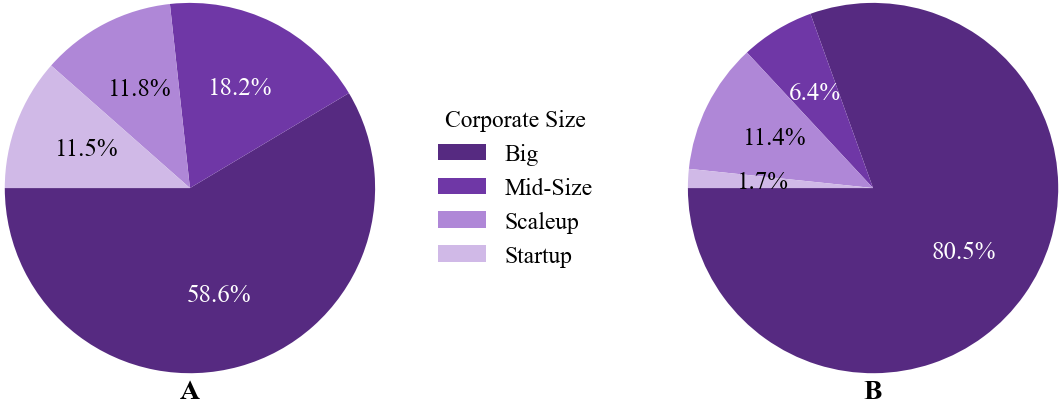
\includegraphics[width=0.75\textwidth]{report/images/pie_charts.png}  
  \caption{Corporate size distribution (A) and paper contributions by corporate size (B) are based on corporate institutions that participated in CVPR, ICCV, and WACV from 2019 to 2024. Large institutions dominate both participation and research output, representing 58.6\% of participating institutions while contributing 80.5\% of the total papers.}
  \vspace{-10pt}
  \label{fig:corporate_size_graph}
\end{figure}

\vspace{-10pt}
\subsection{Research Focus}
\vspace{-7pt}
As seen from Figure \ref{fig:research_focus_radar}, corporate-affiliated research dominates both in the number of papers and citations in hot topics: Generative Models \& Creativity and Natural Language Processing. Corporate
affiliated research also takes the lead in areas like Autonomous Vehicles \& Robotics and Augmented Reality (AR) \& Virtual Reality (VR), highlighting strong corporate investment to applied fields. Additionally, fields essential to progress, such as Datasets \& Benchmarks and Data Collection \& Management, receive attention from corporate research, aligning with the industry's reliance on large-scale proprietary datasets.
\begin{wrapfigure}[28]{r}{0.5\textwidth}
\centering
\vspace{-15pt}
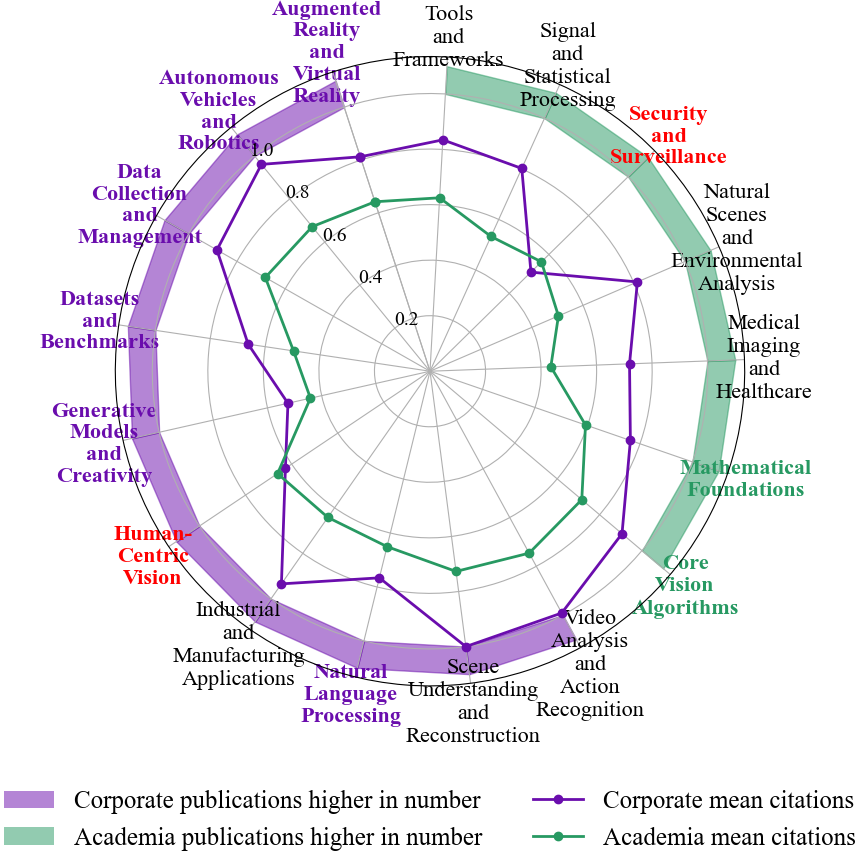
\includegraphics[width=0.5\textwidth]{report/images/citation_radar_plot.png}  
% \caption{Proportion of corporate and academia papers (normalized by the total number of papers from each group) across different categories.}
\caption{Research focus of corporate and academic institutions is shown by shaded areas, based on the number of paper contributions, while impact is represented by lines as mean citation counts (with 1.0 corresponding to 70 citations). Corporate research leads in high-impact areas like Generative Models and NLP, and applied fields such as Autonomous Vehicles \& Robotics and AR/VR, while academia remains influential in Mathematical Foundations and Core Vision Algorithms.}
\label{fig:research_focus_radar}

\end{wrapfigure}
Academia, on the other hand, produces more papers in foundational areas like Mathematical Foundations and Core Computer Vision Algorithms, underscoring its focus on theoretical advancements. However, this higher paper volume does not always translate to greater impact. Corporate research tends to receive more citations, even in fields where academia publishes more. One exception is Security \& Surveillance, where academic research maintains a stronger influence. Similarly, corporate-led fields generally dominate in citations, except for Human-Centric Vision, where academia remains competitive in influence. 
% \vspace{20pt}
\section{Discussion}
\vspace{-7pt}
Our study highlights the increasing presence of corporate-affiliated research in top-tier computer vision conferences. While academia produces more papers, corporate contributions have steadily grown, with corporate co-authored papers receiving higher citation counts on average. This trend is largely driven by a few major technology firms, reflecting their strong influence on the field.

Corporate and academic research priorities also diverge: academia emphasizes Mathematical Foundations and Tools as well as Security and Surveillance, while corporations focus more on applied areas such as Generative Models, Autonomous Vehicles, AR/VR, and Video Analysis. Industry also leads in large-scale dataset collection, reinforcing its advantage in data-driven research.

Our analysis focuses on accepted papers from CVPR (dominating the dataset), ICCV, and WACV, excluding many other conferences and rejected submissions, which may reveal different trends or selection biases. Additionally, citation counts are primarily sourced from IEEE Xplore, potentially overlooking citations from non-IEEE sources, industry reports, and preprints. We also noted that corporate research is geographically concentrated in the USA and China, while academia is distributed globally. Further investigation is needed to understand international corporate research collaboration.

Future studies should explore how corporate funding shapes research priorities and whether this affects inclusivity and diversity in the field. Ethical concerns surrounding proprietary datasets and closed-source models should also be examined, as they impact accessibility and transparency. Additionally, analyzing collaboration patterns between academia and industry could provide insights into fostering sustainable and inclusive research partnerships.
\vspace{-7pt}
\section{Statement of Contribution}
\vspace{-7pt}
All authors contributed to data pre-processing including affiliation categorization and keyword grouping, figure corrections, manuscript writing, proofreading and code management. 

Merve Kocabas analyzed corporate research growth, corporate size distribution, and citation research focus areas. Hari J. A. Senthilprathiban conducted citation analysis and statistical tests. Irem Karaca examined country distributions of affiliations and created the citation density graph. Shubham S. Raheja scraped IEEE Xplore pages and analyzed the dominant groups in research focus areas.

%Merve analysed the growth of corporate-affiliated research and the research focus of academia and industry. Irem analysed the influence of large corporations. Hari conducted the citation count statistical test. Shubham analysed the research focus of academia and industry and scraped IEEE Xplore pages. All authors contributed in categorizing affiliations and keywords of papers, making figures and writing the manuscript.
% Merve analyzed the corporate affiliated paper ratio over time and corporate size and paper distribution and focused on extracting keywords and company and university affiliations for ICCV papers. Irem created the choropleth map analysing academia and corporates by countries and extracting the features for CVPR 2022-2024. Hari conducted the citaion count statistical test and extracted the data for the WACV papers. Shubham created the keyword radar plot, scraped the data from the IEEE papers and extracted the data for CVPR 2019-2021. All members of the group contributed to writing the report.
% This is the last section before the references. 

% \emph{Here is an example:}

% XX performed the correlation analysis, organized the data and code for the processing of dataset1 and subdataset2, and created the scatter plot. 
% YY created the random forest regression model, performed the data cleaning for the xyz analysis / xyz database, and created the bar charts to display the regression results. 
% ZZ researched and collected the raw data, restructured the pipeline for the data analysis, and proof-read the draft for the final report. 
% AA performed the data cleaning for dataset1, and performed the Ridge and Lasso regularization. 
% All members of the group contributed to writing the report.

\newpage
\section*{References}

[1] M. Färber and L. Tampakis, “Analyzing the Impact of Companies on AI Research Based on Publications,” CoRR, vol. abs/2310.20444, 2023, doi: 10.48550/ARXIV.2310.20444.

[2] D. I. Yue, "Google: Estimating the Impact of Corporate Involvement on AI Research," SSRN, Nov. 25, 2024. [Online]. Available: \url{https://ssrn.com/abstract=5033334.} doi: 10.2139/ssrn.5033334.

[3] Google Scholar. Top Publications - Computer Vision & Pattern Recognition. Retrieved February 10, 2025, from \url{https://scholar.google.com/citations?view_op=top_venues&hl=en&vq=eng_computervisionpatternrecognition}

[4] Paper Copilot, "Paper Lists," Retrieved January 3, 2025, from \url{https://github.com/papercopilot/paperlists}

[5] Dun \& Bradstreet. (n.d.). Business directory. Retrieved February 1, 2025, from \url{https://www.dnb.com/business-directory.html}

[6] arXiv. (n.d.). arXiv category taxonomy. arXiv. Retrieved February 1, 2025, from \url{https://arxiv.org/category\textunderscore taxonomy}

[7] T. D. Gauthier, "Detecting Trends Using Spearman's Rank Correlation Coefficient," Environmental Forensics, vol. 2, no. 4, pp. 359-362, 2001. [Online]. Available: \url{https://www.sciencedirect.com/science/article/pii/S1527592201900618.} doi: 10.1006/enfo.2001.0061.

[8] Yue, Sheng \& Pilon, Paul \& Cavadias, George. (2002). Power of the Mann-Kendall and Spearman's Rho Tests For Detecting Monotonic Trends in Hydrological Series. Journal of Hydrology. 259. 254-271. 10.1016/S0022-1694(01)00594-7. 

[9] H. B. Mann and D. R. Whitney, “On a Test of Whether one of Two Random Variables is Stochastically Larger than the Other,” The Annals of Mathematical Statistics, vol. 18, no. 1, pp. 50–60, 1947, doi: 10.1214/aoms/1177730491.
\end{document}